\documentclass{../../slides-style}

\slidetitle{Системы контроля версий}{16.09.2022}

\begin{document}

    \begin{frame}[plain]
        \titlepage
    \end{frame}

    \section{Введение}

    \begin{frame}
        \frametitle{Мотивация}
        \begin{itemize}
            \item Откат изменений
            \begin{itemize}
                \item Система контроля версий --- это машина времени
            \end{itemize}
            \item Управление версиями
            \begin{itemize}
                \item Машина времени с альтернативными временными ветками
            \end{itemize}
            \item Централизованное хранение кода
            \item Командная разработка
        \end{itemize}
    \end{frame}

    \begin{frame}
        \frametitle{Локальные копии}
        \begin{center}
            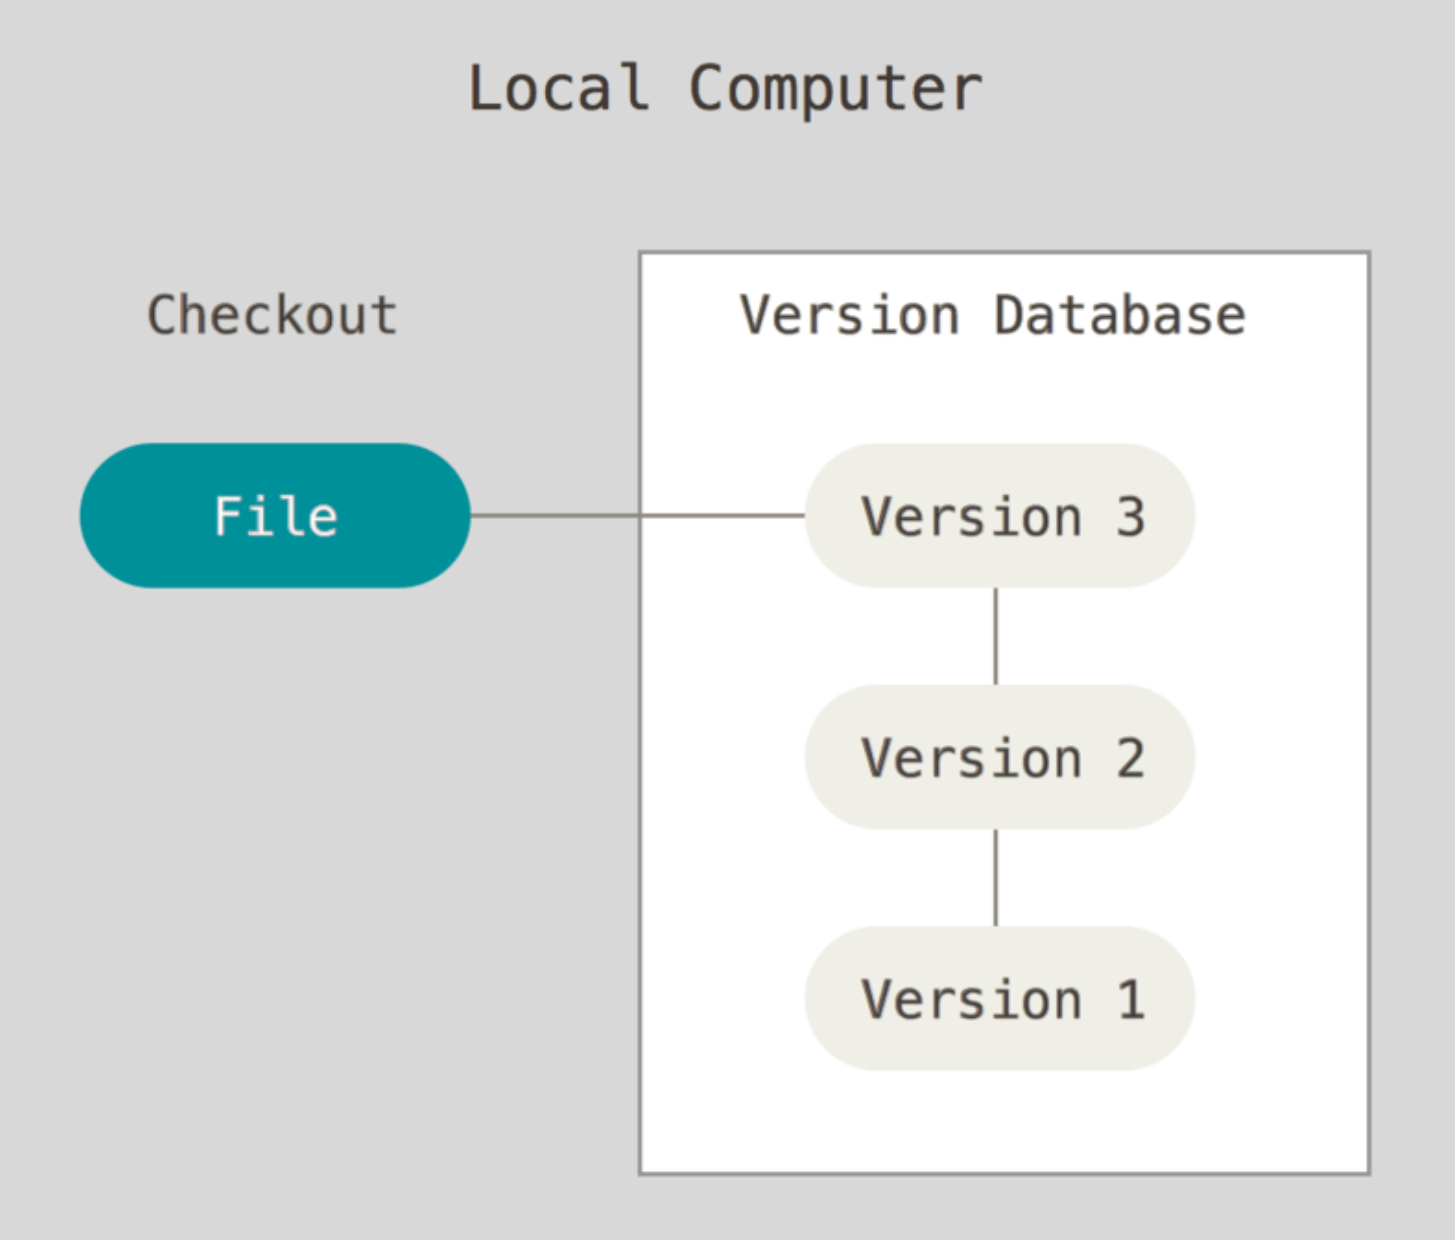
\includegraphics[width=0.6\textwidth]{localCopies.png}
            \attribution{https://git-scm.com/book/ru}
        \end{center}
    \end{frame}

    \begin{frame}
        \frametitle{Централизованные VCS}
        \begin{center}
            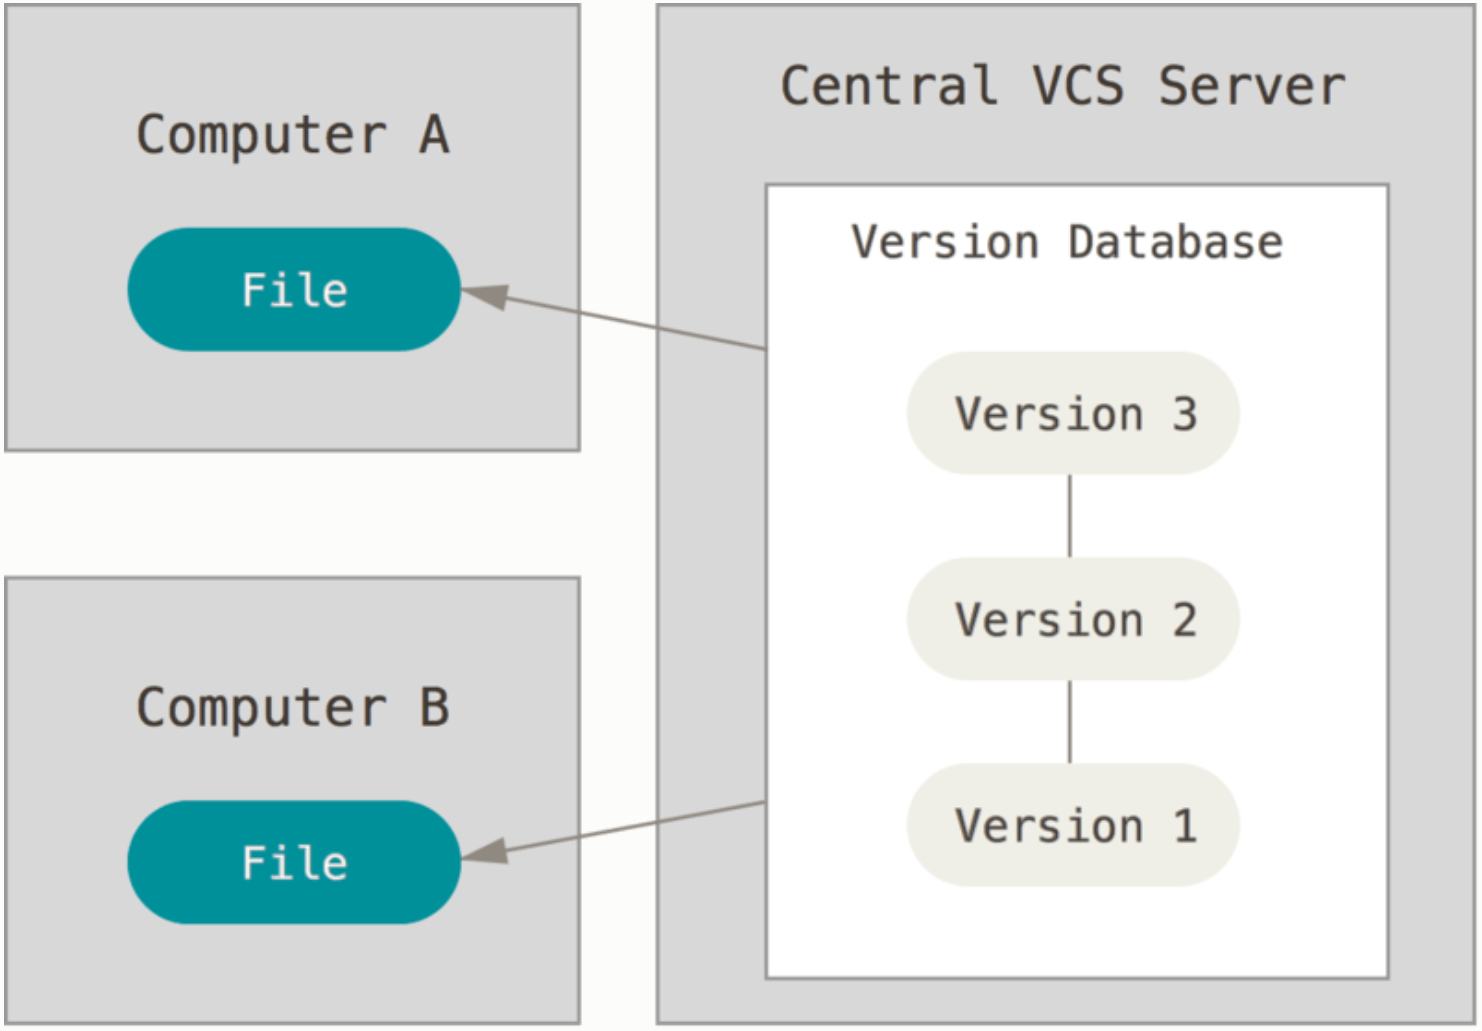
\includegraphics[width=0.6\textwidth]{centralizedVcs.png}
            \attribution{https://git-scm.com/book/ru}
        \end{center}
    \end{frame}

    \begin{frame}
        \frametitle{Распределённые VCS}
        \begin{center}
            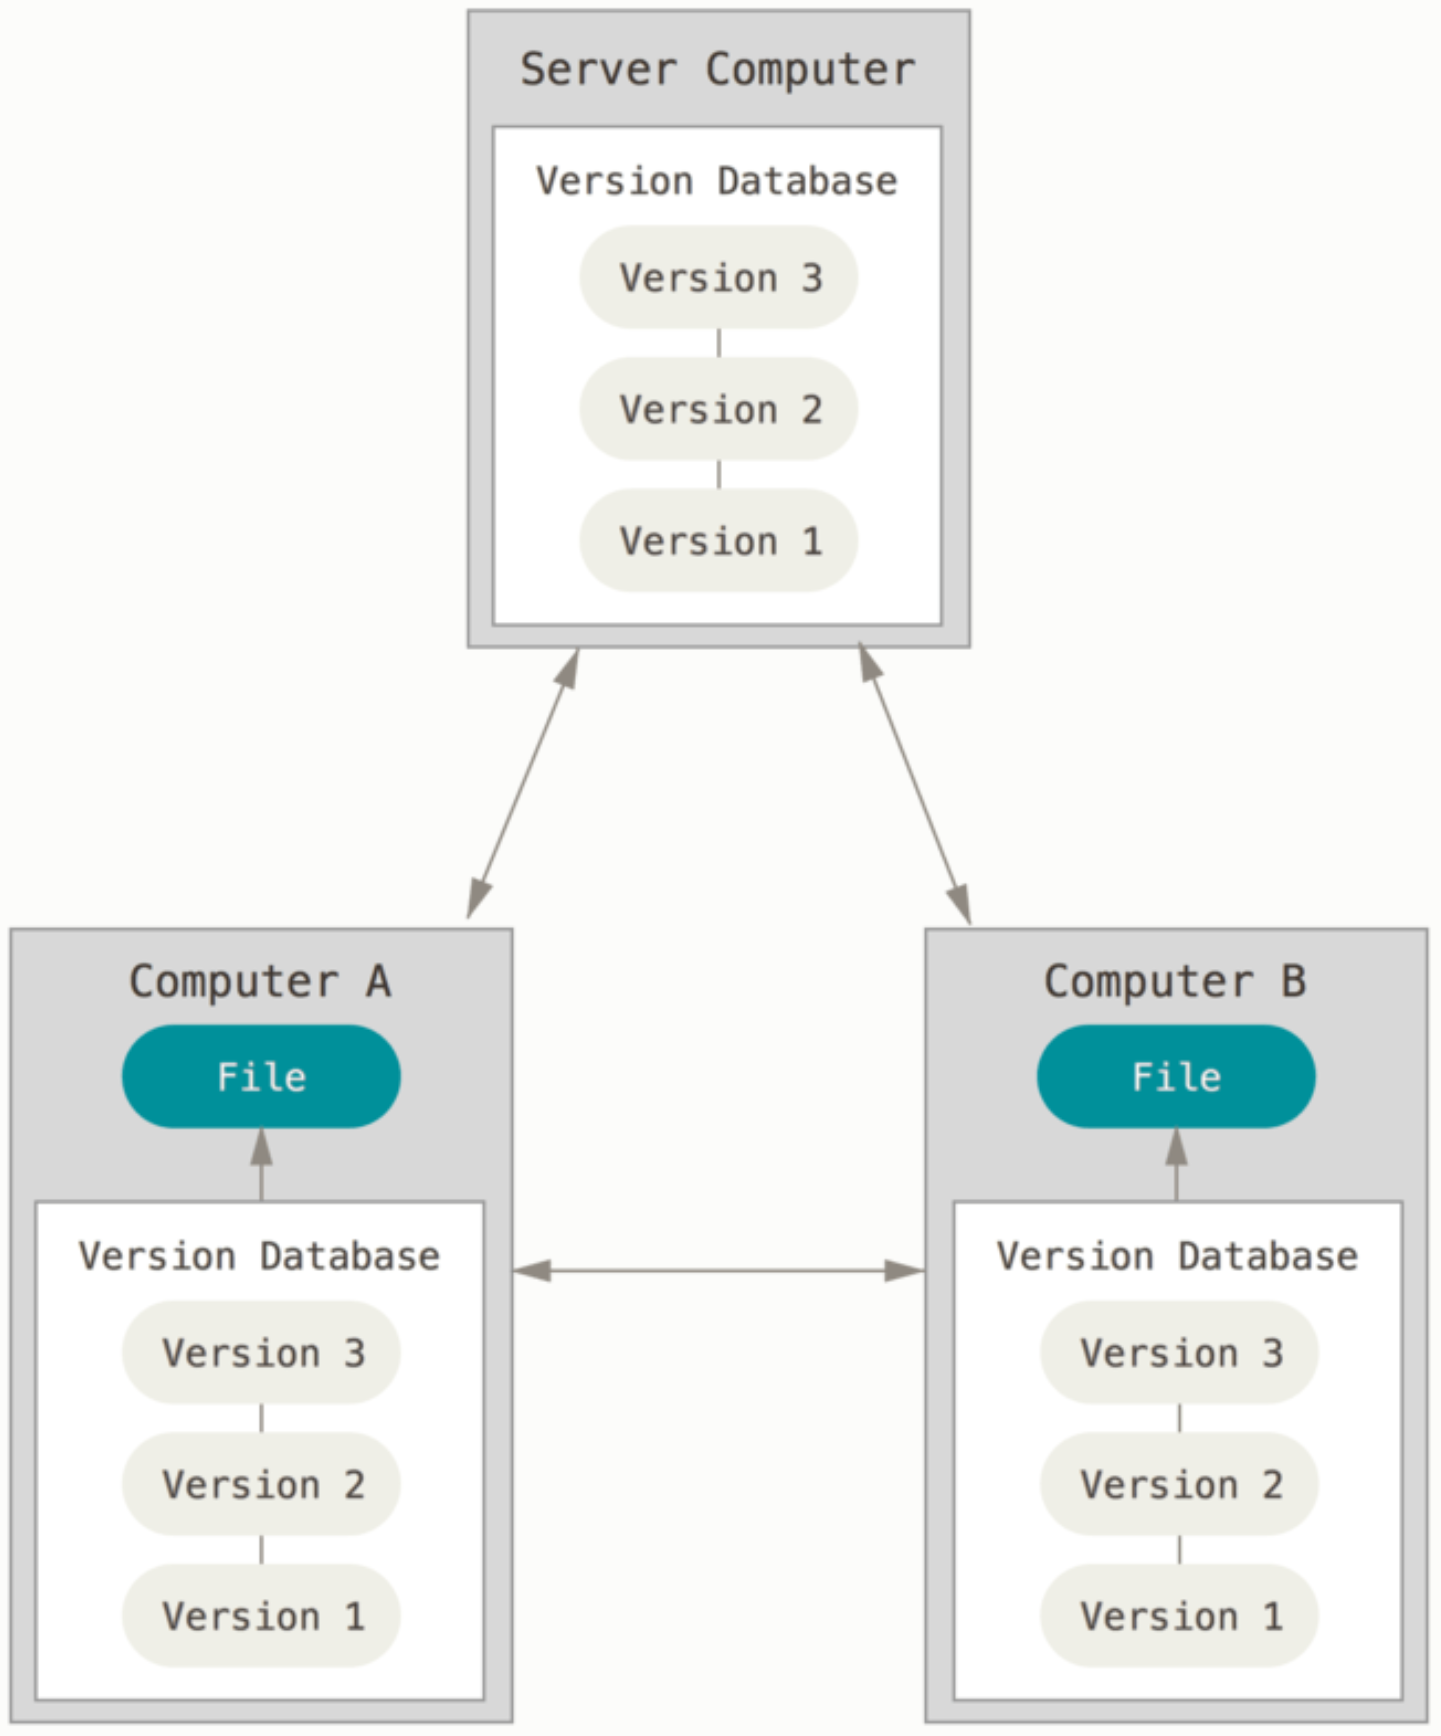
\includegraphics[width=0.4\textwidth]{distributedVcs.png}
            \attribution{https://git-scm.com/book/ru}
        \end{center}
    \end{frame}

    \begin{frame}
        \frametitle{Дельты}
        \begin{itemize}
            \item Системы контроля версий управляют изменениями
            \item Единица работы --- коммит, набор изменений по всем файлам репозитория
            \item Файлы системы контроля версий не очень интересуют!
            \item Рабочая копия --- папка с исходниками, где ведётся разработка
        \end{itemize}
        \begin{center}
            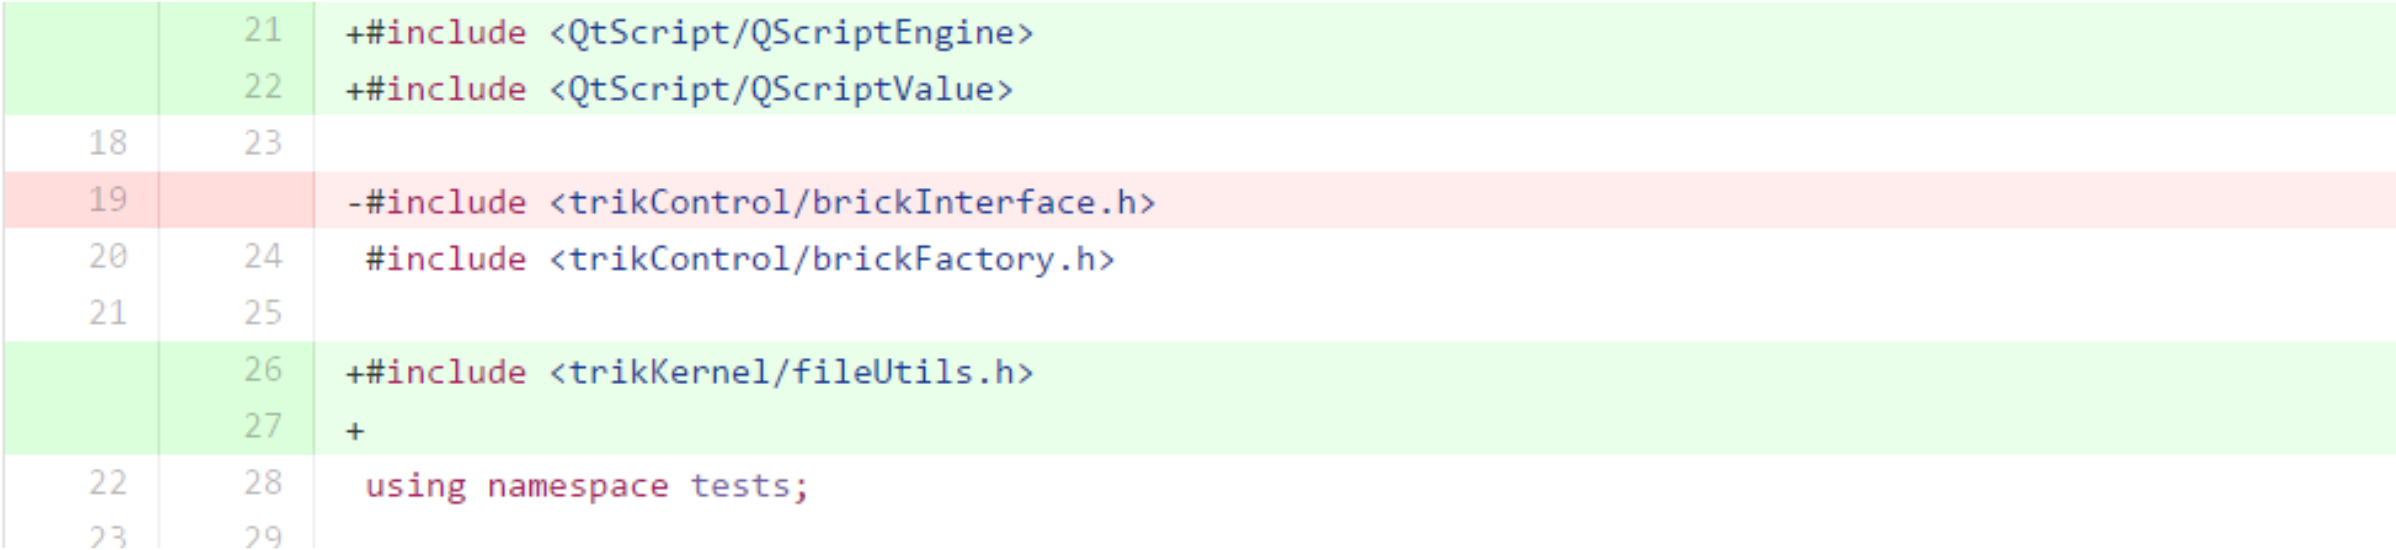
\includegraphics[width=0.8\textwidth]{delta.png}
        \end{center}
    \end{frame}

    \section{Git}

    \begin{frame}
        \frametitle{Конкретно Git}
        \begin{itemize}
            \item Не GitHub!
            \item Не файлообменник
            \item Распределённая система контроля версий
            \item Удобная поддержка веток
            \item 2005 год, Линус Торвальдс (тот самый), для версионирования ядра Linux
            \begin{itemize}
                \item Был написан за несколько дней после ссоры с BitKeeper-ом как набор скриптов на Bash-е
                \item Речь про сотни тысяч коммитов и тысячи коммитеров
            \end{itemize}
            \item С тех пор реализован под все нормальные ОС в виде библиотеки 
            \begin{itemize}
                \item И консольной утилиты, её использующей
            \end{itemize} 
        \end{itemize}
    \end{frame}

    \begin{frame}[fragile]
        \frametitle{Что поставить, чтобы всё работало}
        \begin{itemize}
            \item Git for Windows, \url{https://git-scm.com/download/win}
            \item Linux/MacOS: \verb|apt install git|, \verb|brew install git| или что-то подобное
            \begin{itemize}
                \item Кстати, для Windows есть Chocolatey: \verb|choco install git|
            \end{itemize}
            \item На первое время какой-нибудь графический клиент:
            \begin{itemize}
                \item Github Desktop
                \item TortoiseGit
                \item SmartGit 
                \item ...
                \item Плагин к вашей любимой IDE
            \end{itemize}
        \end{itemize}
    \end{frame}

    \begin{frame}
        \frametitle{Git, жизненный цикл файла}
        \begin{center}
            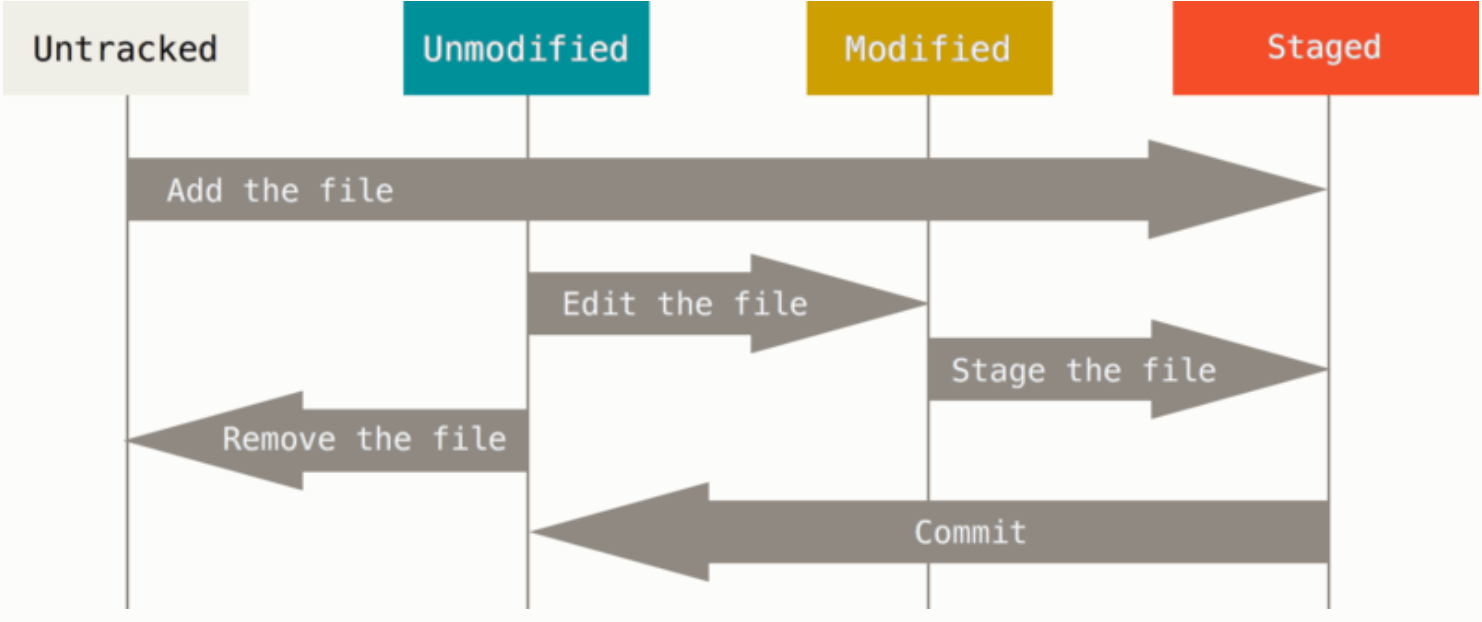
\includegraphics[width=0.8\textwidth]{fileLifeCycle.png}
            \attribution{https://git-scm.com/book/ru}
        \end{center}
    \end{frame}

    \begin{frame}[fragile]
        \frametitle{Основные команды}
        \begin{itemize}
            \item git add --- добавить новый файл под управление git или добавить изменение к коммиту
            \begin{itemize}
                \item Add... в TortoiseGit
            \end{itemize}
            \item git status --- показать список изменённых/добавленных/удалённых файлов
            \begin{itemize}
                \item Diff в TortoiseGit
            \end{itemize}
            \item git diff --- показать изменения по каждому файлу
            \begin{itemize}
                \item В окне Diff двойным кликом по файлу в TortoiseGit
            \end{itemize}
            \item git commit --- зафиксировать изменения, создав новый коммит
            \begin{itemize}
                \item Git Commit в TortoiseGit
            \end{itemize}
            \item git log --- просмотреть список коммитов
            \begin{itemize}
                \item Show log в TortoiseGit
            \end{itemize}
            \item git restore --- откатить изменения в файле или перейти на другую ветку
            \begin{itemize}
                \item Revert... или Switch/Checkout
                \item Есть ещё \verb|git reset --hard|, плюс \verb|git clean -dfx|
            \end{itemize}
        \end{itemize}
    \end{frame}

    \begin{frame}
        \frametitle{Демо}
        \begin{itemize}
            \item Надо скачать и поставить консольный клиент Git и TortoiseGit
            \item Создадим локально репозиторий, научимся коммитить файлы, смотреть историю и откатывать изменения
        \end{itemize}
    \end{frame}

    \begin{frame}[fragile]
        \frametitle{Ветки}
        \begin{itemize}
            \item Ветка --- цепочка коммитов
            \item История коммитов может ветвиться, как дерево
            \begin{itemize}
                \item Хотим проверить вариант решения
                \item Хотим не выкладывать в основную ветку недоделанную работу
                \item Хотим при командной разработке не мешать друг другу
            \end{itemize}
            \item \verb|git checkout -b <имя ветки>| --- отвести новую ветку от текущей
            \item \verb|git checkout <имя ветки>| --- переключиться на указанную ветку
            \begin{itemize}
                \item Switch/Checkout в TortoiseGit, там же флажок Create New Branch
            \end{itemize}
            \item Очень важно следить, от какой ветки отводим новую
        \end{itemize}
    \end{frame}

    \begin{frame}[fragile]
        \frametitle{Слияние веток}
        \verb|git merge <имя ветки>| --- притянуть изменения из указанной ветки в текущую
        \begin{minted}{text}
            $ git checkout master
            $ git merge iss53
        \end{minted}
        \begin{center}
            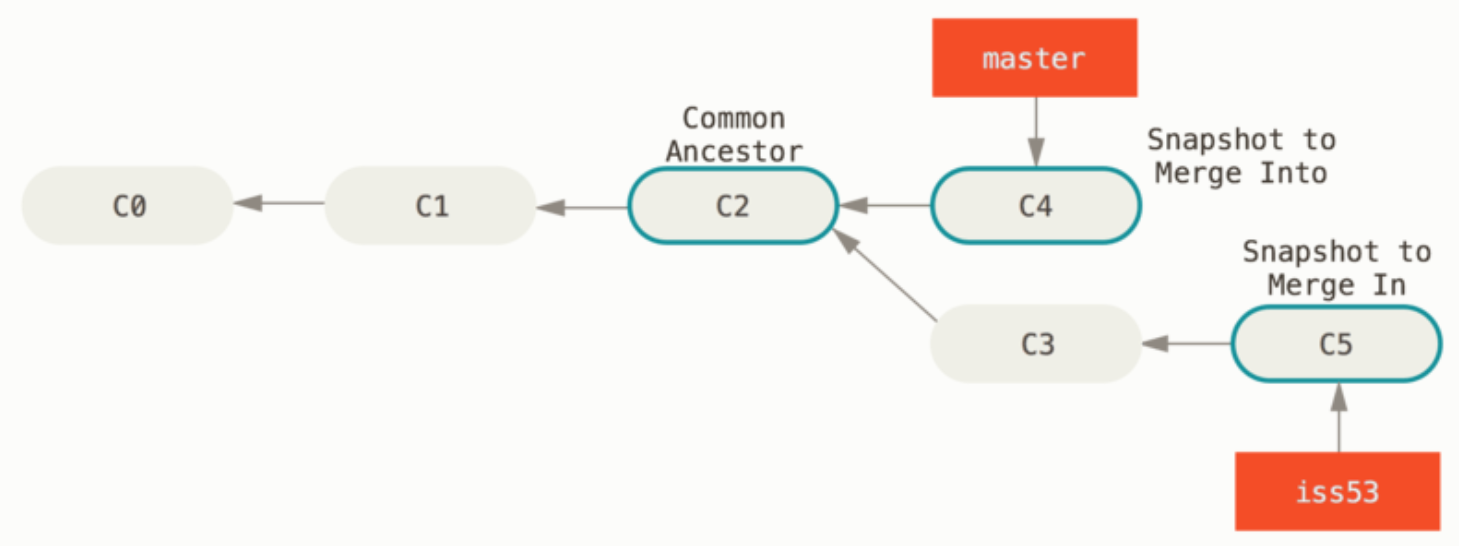
\includegraphics[width=0.7\textwidth]{merge.png}
        \end{center}
        \begin{center}
            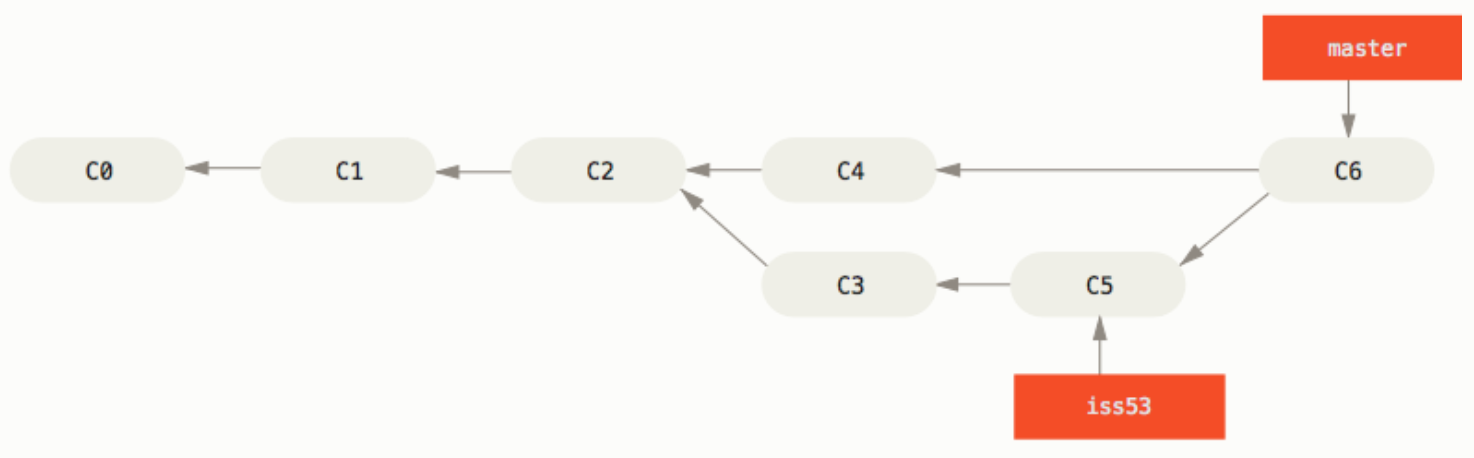
\includegraphics[width=0.7\textwidth]{mergeResult.png}
            \attribution{https://git-scm.com/book/ru}
        \end{center}
    \end{frame}

    \begin{frame}
        \frametitle{Конфликты}
        \begin{center}
            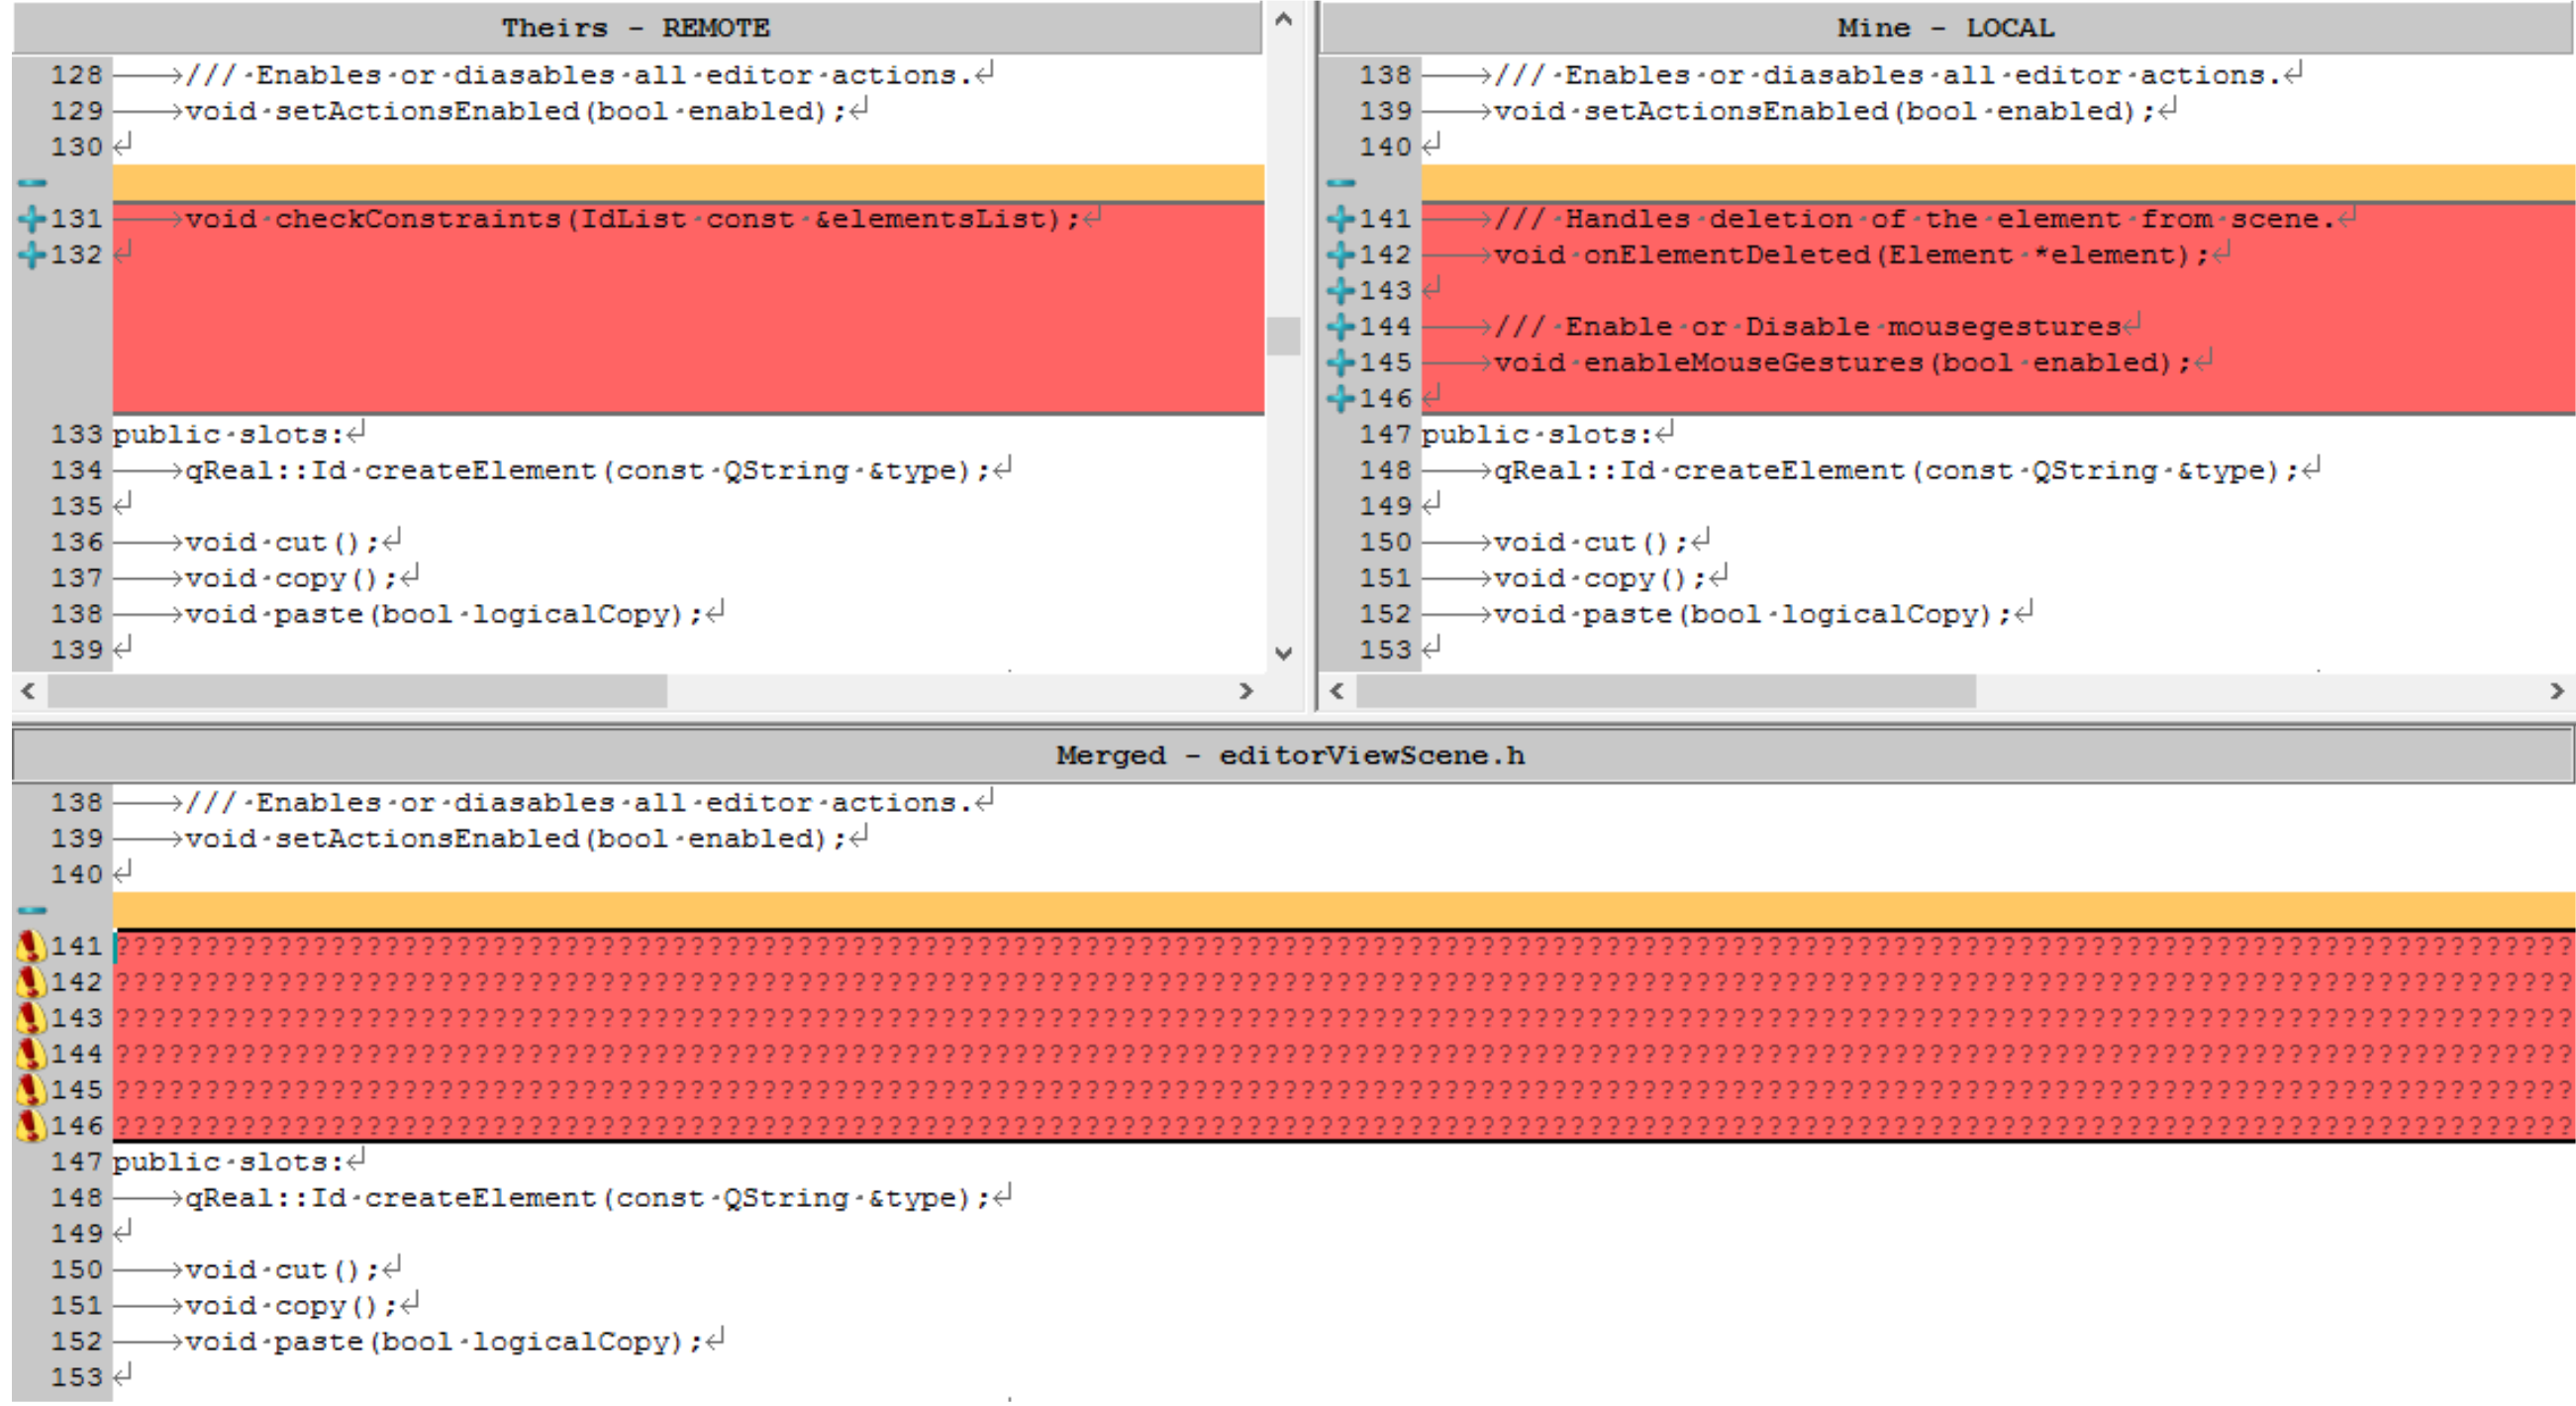
\includegraphics[width=0.7\textwidth]{conflicts.png}
        \end{center}
        \begin{center}
            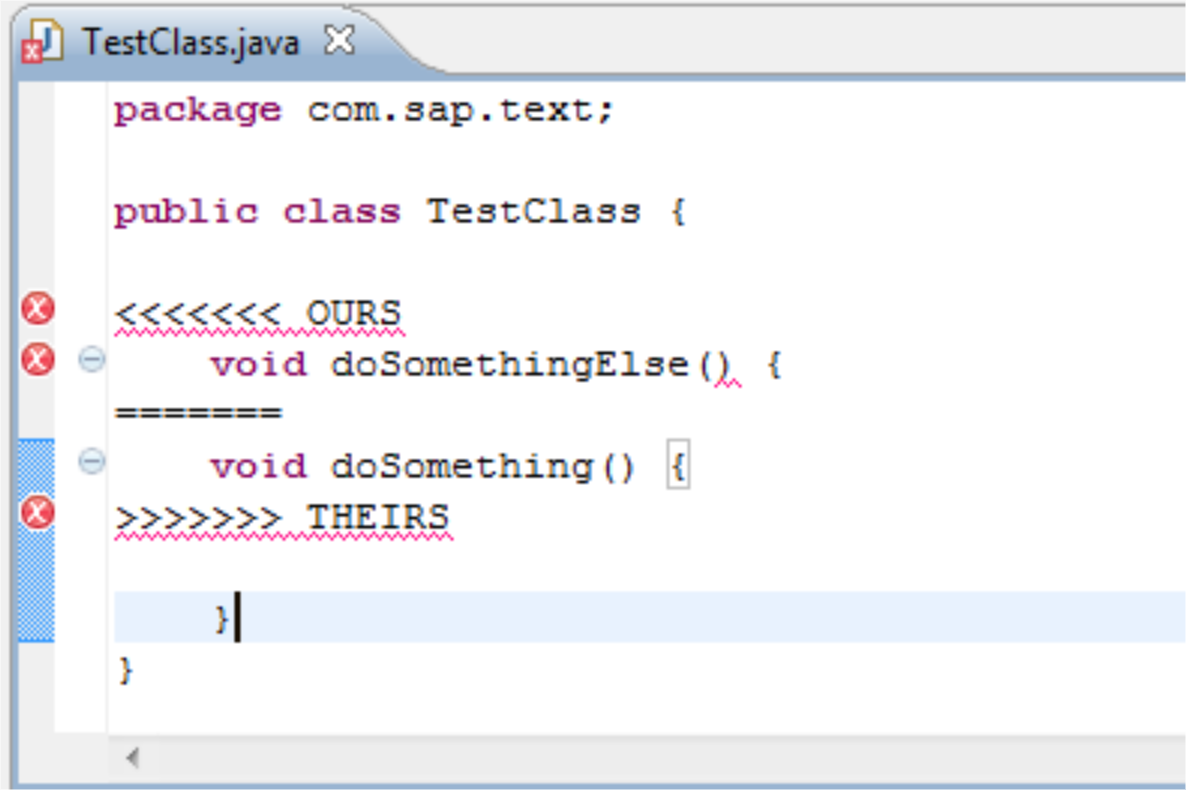
\includegraphics[width=0.3\textwidth]{conflictsInCode.png}
        \end{center}
    \end{frame}

    \begin{frame}
        \frametitle{Удалённые репозитории}
        \begin{columns}
            \begin{column}{0.4\textwidth}
                \begin{itemize}
                    \item git clone
                    \item git remote
                    \item git push
                    \item git fetch
                    \item git pull
                \end{itemize}
            \end{column}
            \begin{column}{0.6\textwidth}
                \begin{center}
                    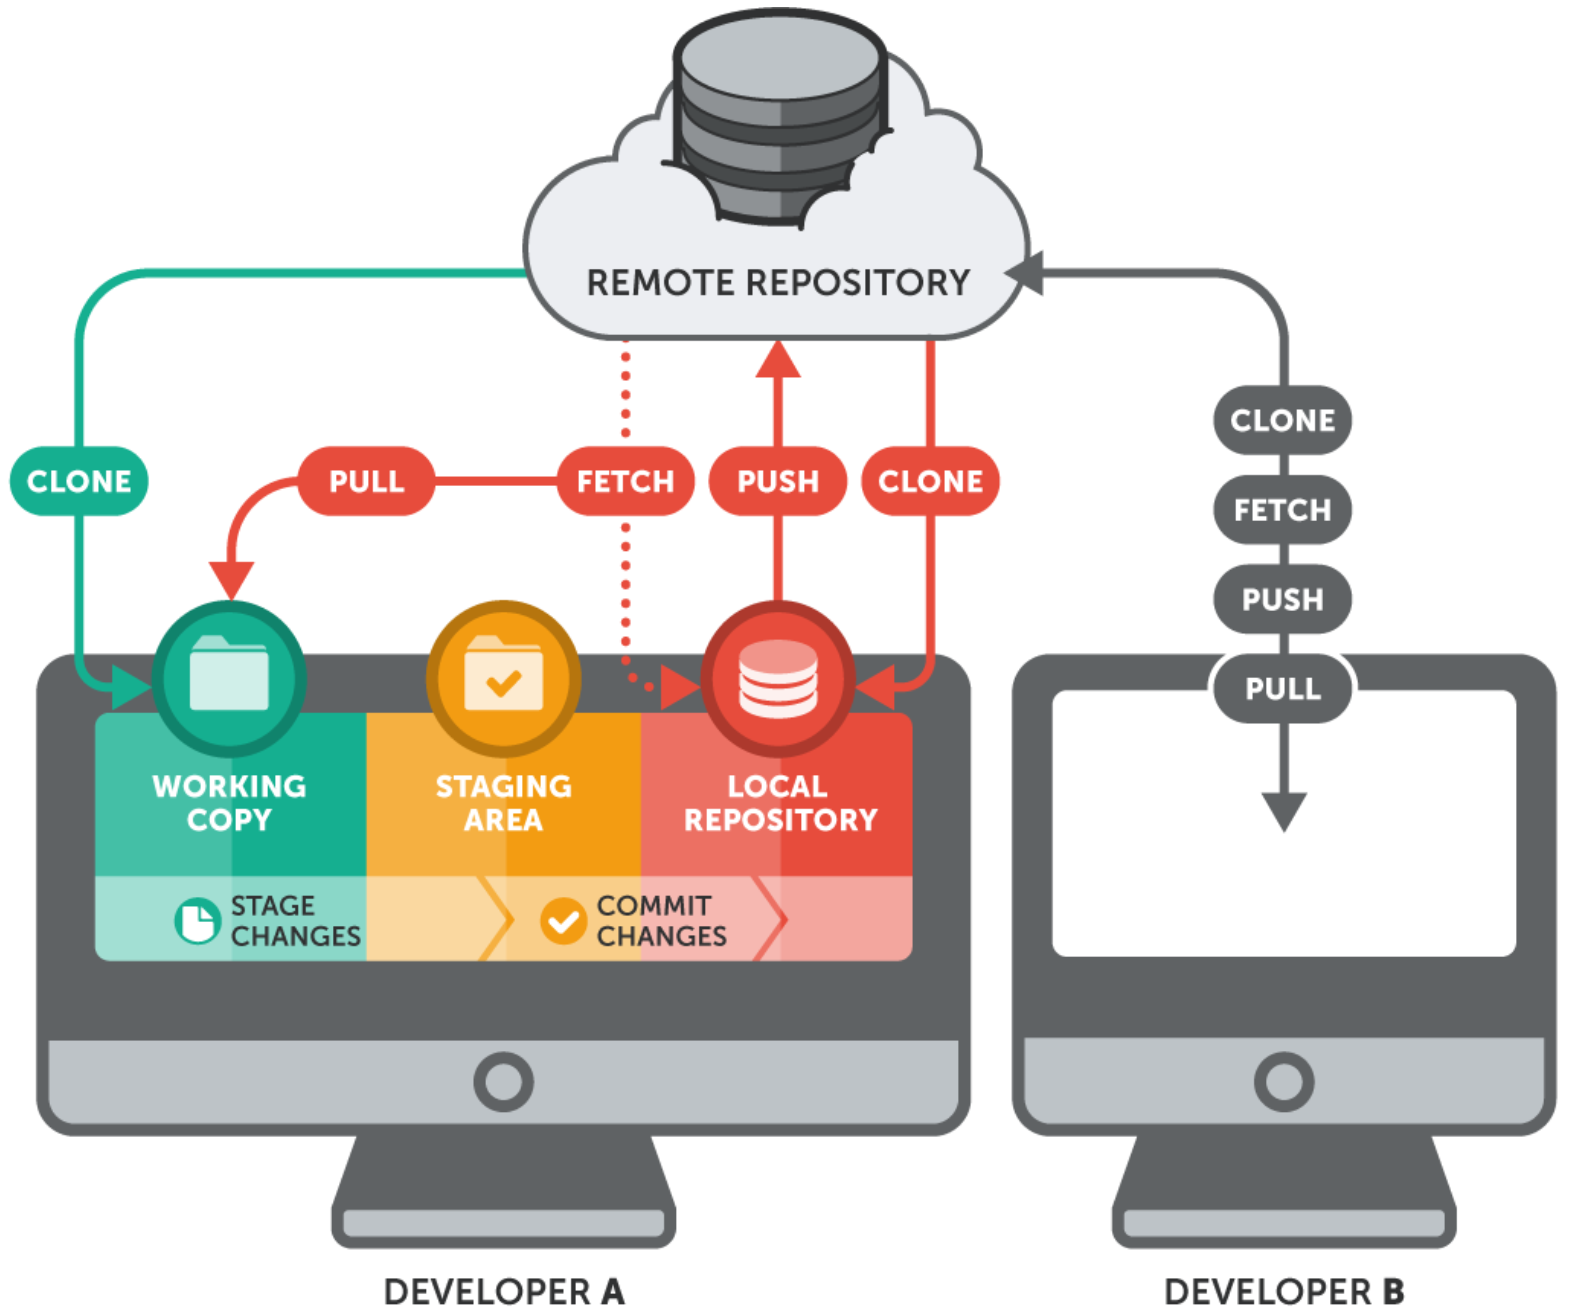
\includegraphics[width=0.95\textwidth]{remoteRepos.png}
                    \attribution{https://www.git-tower.com/learn/git/ebook/en}
                \end{center}
            \end{column}
        \end{columns}
    \end{frame}

    \section{GitHub}

    \begin{frame}
        \frametitle{GitHub}
        \begin{itemize}
            \item GitHub --- один из облачных хостингов git-репозиториев
            \begin{itemize}
                \item Никто не мешает использовать Git локально или поднять сервер самому
            \end{itemize}
            \item Ещё из известных GitLab (включая self-hosted), BitBucket, Azure DevOps Server, ...
            \item Не только хостинг репозитория, но и:
            \begin{itemize}
                \item UI для просмотра исходников и поиска по ним
                \item Пуллреквесты
                \item Форки
                \item Социальное взаимодействие
                \item CI/CD
                \item Средства для управления проектом
            \end{itemize}
        \end{itemize}
    \end{frame}

    \begin{frame}
        \frametitle{Демо}
        \begin{itemize}
            \item Регистрируемся на GitHub
            \item Создаём репозиторий прямо на GitHub
            \item Клоним его себе
            \item Отводим ветку под домашку
            \item Делаем её там
            \item Коммитим/пушим
            \item Делаем пуллреквест в main
        \end{itemize}
    \end{frame}

    \begin{frame}
        \frametitle{Процесс работы}
        \begin{footnotesize}
            \begin{itemize}
                \item Программист хочет сделать новую фичу
                \item Отводит себе ветку от main-а
                \item Реализует там фичу
                \item Тестит и рефакторит её, когда считает, что она готова, делает пуллреквест
                \item Пока пуллреквест ревьюят, программист делает новую фичу (опять-таки, отведя новую ветку от main-а)
                \item По пуллреквесту появляются замечания, программист переключается на ветку пуллреквеста и правит там замечания
                \item Когда поправил, коммитит и пушит исправления, они автоматом добавляются в пуллреквест
                \item Просит ревьюеров, чтобы они посмотрели фиксы
                \item Переключается обратно на свою рабочую ветку и продолжает писать код, возможно, делая ещё пуллреквесты 
                \item Цикл повторяется до тех пор, пока пуллреквест не принимают
                \item Программист удаляет ветку с фичей, когда она замерджена
            \end{itemize}
        \end{footnotesize}
    \end{frame}

    \begin{frame}
        \frametitle{Git Flow}
        \begin{center}
            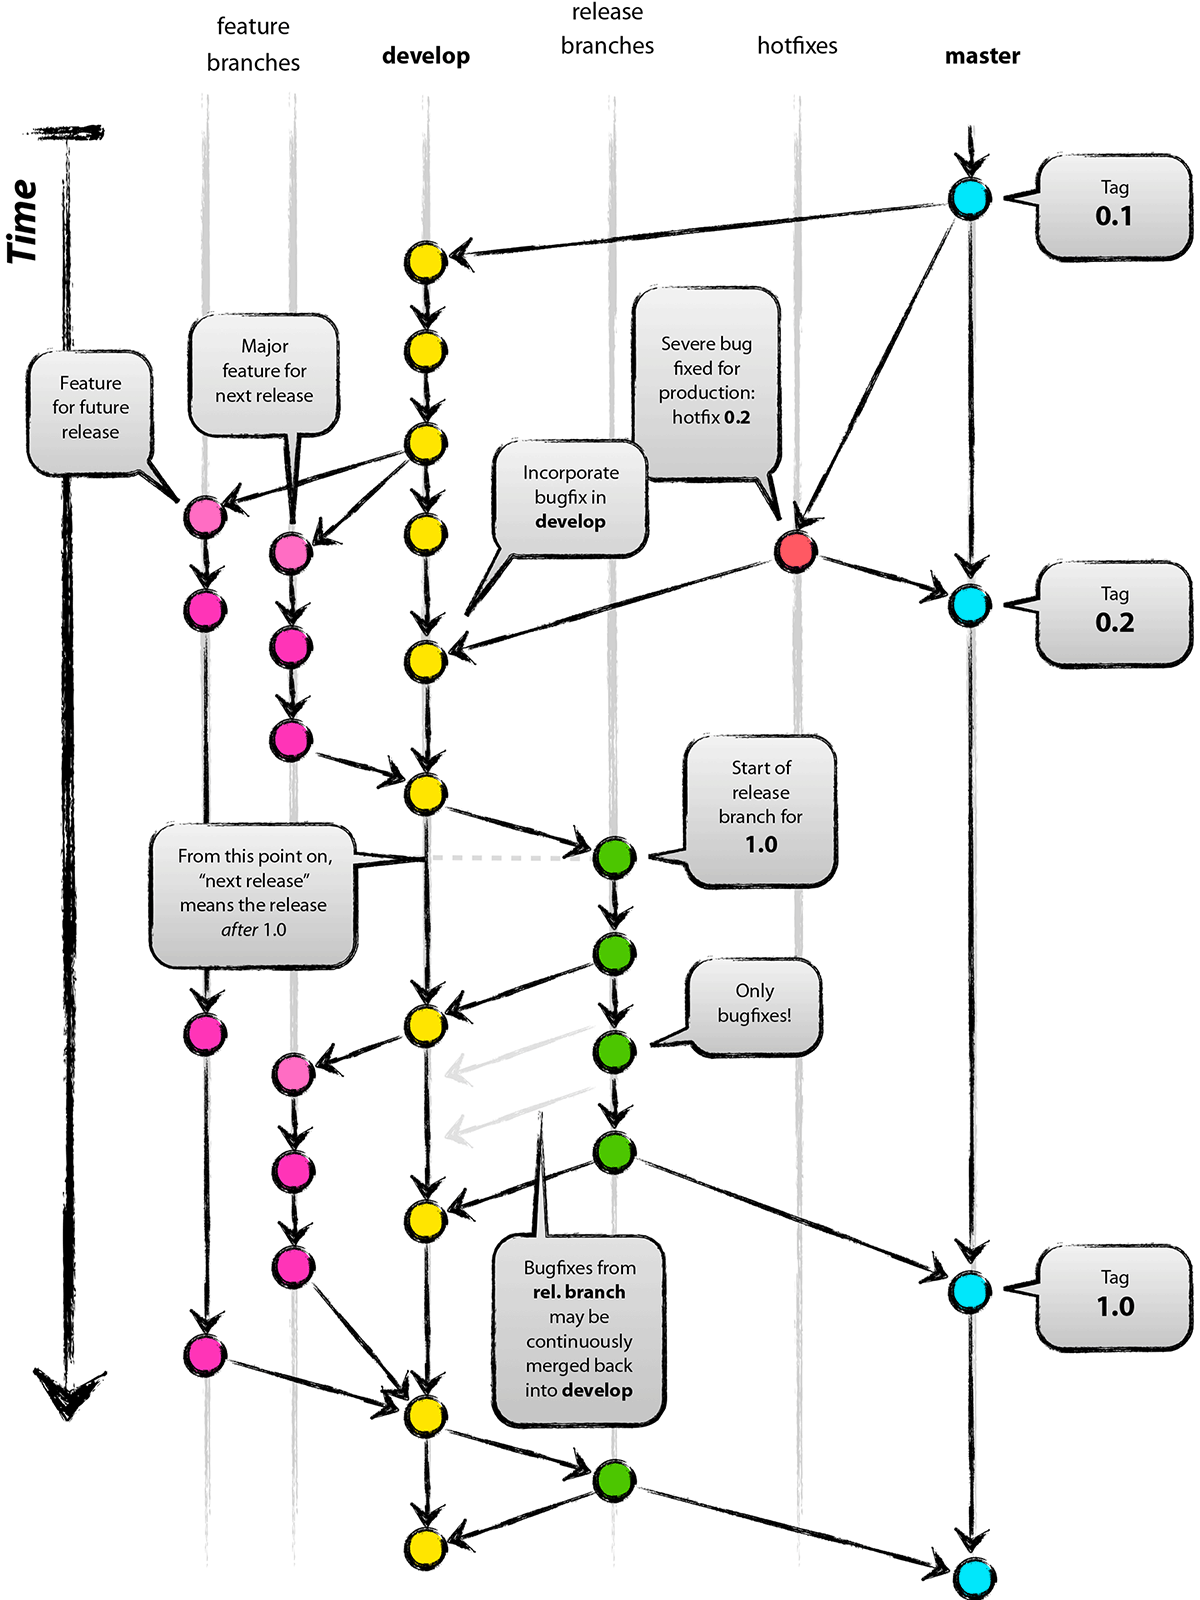
\includegraphics[width=0.42\textwidth]{gitFlow.png}
            \attribution{https://nvie.com/posts/a-successful-git-branching-model/}
        \end{center}
    \end{frame}

    \section{Хорошие практики}

    \begin{frame}
        \frametitle{Хорошие практики}
        \begin{itemize}
            \item Коммитим только исходные тексты, конфиги, картинки и т.п.
            \item Если что-то может быть автоматически сгенерировано по тому, что уже есть в репозитории, это НЕ коммитим
            \item Всегда пишем адекватные комментарии к коммитам
            \begin{itemize}
                \item Одно-два осмысленных предложения, в повелительной форме
                \item Комментарии к коммиту обязательны, за fix или ``.'' сразу увольняют
            \end{itemize}
            \item Коммитим как можно чаще
            \begin{itemize}
                \item Сделали что-то осмысленное --- коммит
            \end{itemize}
        \end{itemize}
    \end{frame}

    \begin{frame}
        \frametitle{Хорошие практики (2)}
        \begin{itemize}
            \item Никогда не коммитим исполнимые файлы (включая .dll/.so), объектные файлы, локальные настройки
            \begin{itemize}
                \item Из каждого правила есть исключения, но всё же
            \end{itemize}
            \item Обязательно выкладываем файлы, необходимые для сборки
            \begin{itemize}
                \item Проектные файлы, мейкфайлы, скрипты и т.п.
                \item Visual Studio: .vcxproj, .sln
                \item IDEA: всё содержимое папки .idea, кроме workspace.xml и tasks.xml
            \end{itemize}
            \item Имеет смысл проверить, склонив репозиторий в пустую папку
            \begin{itemize}
                \item Кстати, никто не запрещает иметь локально несколько копий репозитория, например, с разными ветками
            \end{itemize}
        \end{itemize}
    \end{frame}

    \begin{frame}
        \frametitle{Хорошие практики (3)}
        \begin{itemize}
            \item Коммит не должен содержать в себе файлы, не относящиеся к изменениям
            \begin{itemize}
                \item .gitignore
                \item \url{https://github.com/github/gitignore}
                \item Обязательно надо проверять, что коммитим (git diff)
            \end{itemize}
            \item Коммит не должен добавлять/убирать пустые строки, менять пробелы на табы и т.д., если это не суть коммита
            \item Стиль исходного кода и отступов должен совпадать с текстом вокруг
            \item Делаете пуллреквест --- посмотрите diff
        \end{itemize}
        \begin{center}
            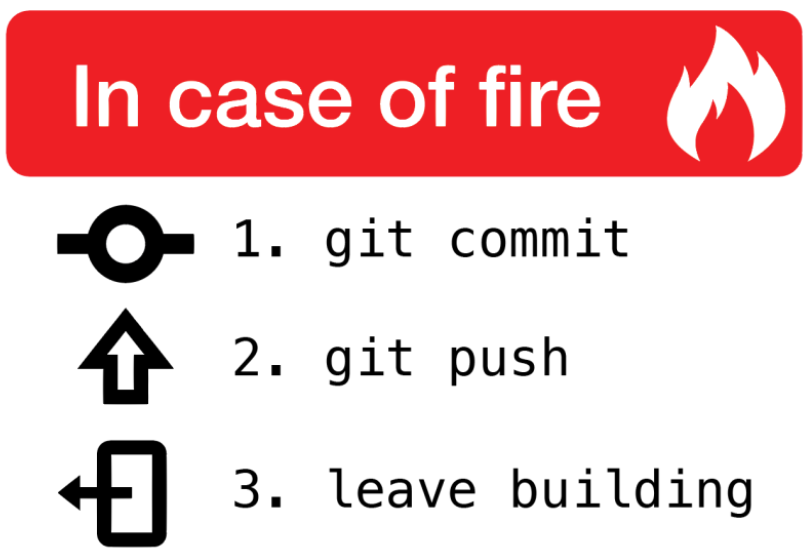
\includegraphics[width=0.4\textwidth]{inCaseOfFire.png}
        \end{center}
    \end{frame}

    \begin{frame}[fragile]
        \frametitle{Ещё полезные команды}
        \begin{itemize}
            \item \verb|git add -p| --- интерактивное добавление изменений к коммиту, позволяет коммитить только часть файла
            \item \verb|git commit --amend| --- исправить последний коммит
            \begin{itemize}
                \item \verb|git commit --amend -m "an updated commit message"|
                \item Применять \textbf{только до} git push
            \end{itemize}
            \item \verb|git rebase <имя ветки>| --- положить изменения из данной ветки поверх текущей, альтернатива merge
            \item \verb|git reset --hard| --- откатить все изменения в рабочей копии до последнего коммита
            \begin{itemize}
                \item Обязательно проверить git status, что не откатите лишнего
            \end{itemize}
            \item \verb|git reset --hard <хеш коммита>| --- откатить все изменения в текущей ветке до указанного коммита, забыть все коммиты, что были после
            \begin{itemize}
                \item И случайно грохнуть всю домашку перед зачётом
            \end{itemize}
        \end{itemize}
    \end{frame}

\end{document}
